\documentclass[letterpaper,11pt]{article}
\pdfoutput=1

\usepackage[margin=2cm]{geometry}
\usepackage{graphicx}
\usepackage{subfig}

\newcommand{\selected}{{\ensuremath s}}
\newcommand{\unselected}{{\ensuremath\slash\!\!\!\selected}}
%\newcommand{\tot}{{\ensuremath\mathrm{tot}}}
\newcommand{\tot}{0}

\begin{document}

\begin{figure}
  \centering
  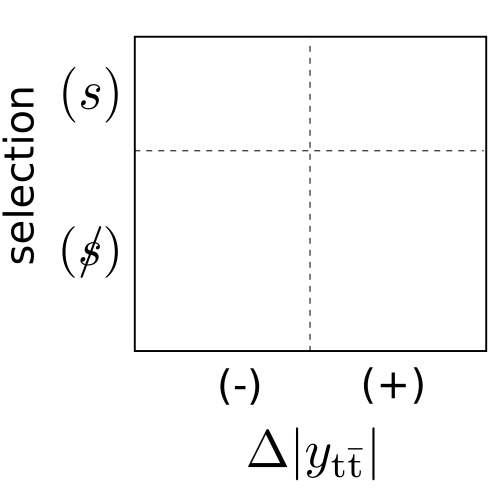
\includegraphics[width=0.3\linewidth]{axes}
  \caption{\label{axes} Four bins, selected ($\selected$) and unselected ($\unselected$) on
    the selection axis, and $(-)$ and $(+)$ on the axis of the the
    observable for which the asymmetry is of interest.}
\end{figure}

Consider a two dimensional distribution of four bins, where one axis
is a selection observable with bins (selected, $\selected$) and
(unselected, $\unselected$), and the other is an observable for which
the asymmetry is of interest, for example
$\Delta|y_{\mathrm{t\bar{t}}}|$, with bins $(+)$ and $(-)$.  Figure
\ref{axes} shows the axes. In a model $N$, the selection contains
$N_\selected=N_\selected^-+N_\selected^+$ events and has asymmetry
$\alpha_\selected$, while the unselected events number
$N_\unselected=N_\unselected^-+N_\unselected^+$ and may have a
different asymmetry $\alpha_\unselected$.  The counts in each bin are
given by
\[N_x^{\pm} = N_x(1\pm\alpha_x)/2,\qquad x\in\{\selected,\unselected\}\]
and the total asymmetry is given by
\[\alpha_\tot = \frac{N_\selected\alpha_\selected + N_\unselected\alpha_\unselected}{N_\selected+N_\unselected}.\]
Note that $\alpha_\selected\ne\alpha_\unselected$ if and only if the selection
efficiencies for the bins $(+)$ and $(-)$ are unequal.

\section{Two families of models}

Consider a two families of models of which $N$ is a member.  The
models $T(f)$ have an antisymmetric component proportional to that of
model $N$, with factor $f$,
\[T_x^{\pm}(f) = N_x(1\pm f\alpha_x)/2,\qquad x\in{\selected,\unselected,\tot}.\]
The asymmetries of a model $T(f)$ would be
\[\alpha_x^{(T)}=f\alpha_x, \qquad x\in\{\selected,\unselected,\tot\}.\]
The other family of models $U(w^\pm)$ is given by uniform reweighting
of the $(\pm)$ bins,
\[U_x^\pm(w^\pm) = N_x^\pm w^\pm(\mathrm{normalization\ constant}).\]
For simplicity of discussion, we will suppose $w^\pm=1\pm k$, but this
will not restrict the generality of our results.  Then
\[U_x^\pm(k) = \frac{N_x}{2}\left(\frac{1+k\alpha_x}{(1+k\alpha_\tot)}\pm\frac{\alpha_x+k}{1+k\alpha_\tot}\right), \qquad x\in\{\selected,\unselected,\tot\}.\]
The asymmetries of a model $U(k)$ would be
\[\alpha_x^{(U)} = \frac{\alpha_x+k}{1+k\alpha_x}, \qquad x\in\{\selected,\unselected,\tot\}.\]
In the general case $\alpha_\selected\ne\alpha_\unselected$, the
intersection of families $T(f)$ and $U(k)$ is $N=T(1)=U(0)$.  Some
notable features of each family of models include:
\begin{description}
\item[Models $T$]:
  \begin{itemize}
  \item Constant asymmetry proportions $\alpha_\tot^{(T)}:\alpha^{(T)}_\selected:\alpha^{(T)}_\unselected$
  \item Constant global selection ratio $T_\selected:T_\unselected$
  \item Variable bin selection ratios $T^\pm_\selected:T^\pm_\unselected$
  \end{itemize}
\item[Models $U$]:
  \begin{itemize}
  \item Constant bin selection ratios $U^\pm_\selected:U^\pm_\unselected$
  \item Variable global selection ratio $U_\selected:U_\unselected$
  \item Variable asymmetry proportions $\alpha_\tot^{(U)}:\alpha^{(U)}_\selected:\alpha^{(U)}_\unselected$
  \end{itemize}
\end{description}


\section{Extrapolation of total asymmetry from observations}

Suppose we wish to calculate the total asymmetry of a sample $D$ from
the observation of its selected components
$D_\selected^\pm=N_\selected(1\pm\alpha^{(D)}_\selected)/2$, based on
the model $N$.  We will generally find different results depending on
our hypothesis concerning which family of models, $T$ or $U$, better
describes $D$.  Supposing $D$ belongs to family $T$, we use the
property of constant ratio $\alpha_\tot/\alpha_\selected$ to
extrapolate the total asymmetry (template method), finding
\[[T]: \alpha_\tot^{(D)} = \left(\frac{\alpha_\tot}{\alpha_\selected}\right)\alpha^{(D)}_\selected.\]
Supposing $D$ belongs to family $U$ on the other hand, we use the
property of constant bin selection efficiencies to extrapolate total
asymmetry (unfolding method), finding
\[[U]: \alpha_\tot^{(D)} = \frac{\alpha^{(D)}_\selected(1-\alpha^2_\selected)N_\selected/N_\unselected + \alpha^{(D)}_\selected(1-\alpha_\selected\alpha_\unselected)+(\alpha_\unselected-\alpha_\selected)}{
                                                       (1-\alpha^2_\selected)N_\selected/N_\unselected + (1-\alpha_\selected\alpha_\unselected)+\alpha^{(D)}_\selected(\alpha_\unselected-\alpha_\selected)}{}.\]
%
Extrapolated total asymmetries using the template and unfolding
methods are shown as a function of selection asymmetry in the
observable $\Delta|y_{\mathrm{t\bar{t}}}|$ in Figure \ref{plot}, based
on a CMS lepton+jets selection ($\sim10\%$ efficient) of
$\mathrm{t\bar{t}}$ events generated by POWHEG, for which the total
asymmetry is $0.56\%$, and the selection asymmetry is $0.32\%$.
\begin{figure}
  \centering
  \includegraphics[width=0.7\textwidth]{plot}
  \caption{\label{plot} Extrapolation of the total asymmetry $A_c^y$
    as a function of the asymmetry of the observable
    $\Delta|y_{\mathrm{t\bar{t}}}|$ in a CMS lepton+4jets selection
    ($\sim$10\% efficient), using two different 2-bin methods based on
    {\sc POWHEG} $\mathrm{t\bar{t}}$ simulation, and asumming perfect
    resolution.  The bisector shows what the extrapolation would be if
    the asymmetry were expected to be selection independent.  Both
    extrapolation methods reduce to the bisector in the case that
    $\alpha_\selected=\alpha_\unselected=\alpha_\tot$, which is not
    the case for POWHEG.}
\end{figure}
These three numbers (total asymmetry, selection asymmetry, selection
efficiency) from any simulation are sufficient to generate the
extrapolation curves for 2-bin versions of both the template method
and the unfolding method.  Clearly the two methods coincide in their
extrapolations only for an observed selection asymmetry equal to that
modeled by the simulation, and diverge quite rapidly from that
intersection.

%\subsection{Template Strategy}
%Following the template strategy we have so far employed, the weights
%which symmetrize and antisymmetrize the original distribution after
%integrating over the selection axis would be
%\[W^\pm_{\mathrm{symm}} = (1\pm\alpha)^{-1},\]
%\[W^\pm_{\mathrm{anti}} = \pm\alpha(1\pm\alpha)^{-1}.\]
%The templates for the selection would be
%\[T^{\pm}_{\mathrm{symm}} = \frac{N_\selected}{2}\frac{1\pm\alpha_\selected}{1\pm\alpha},\]
%\[T^{\pm}_{\mathrm{anti}} = \pm\alpha\frac{N_\selected}{2}\frac{1\pm\alpha_\selected}{1\pm\alpha},\]
%and the parametrized template model would be
%\[T^{\pm}(f) = T^{\pm}_{\mathrm{symm}} + f\cdot T^\pm_{\mathrm{anti}} = \frac{N_\selected}{2}\frac{1\pm\alpha_\selected}{1\pm\alpha}(1\pm f\cdot\alpha).\]
%Our expectation has been that $T^\pm(f) = T^\pm_\selected$ when $f=F$, but
%that is clearly only the case if $F=f=1$ or $\alpha=\alpha_\selected$.  The
%former condition is useless for a measurement, while the latter
%condition is generally unmet, and is particularly untrue in the cases
%of our subselections at extremes of $\mathrm{t\bar{t}}$ system
%rapidity and mass.
%

\section{Argument for Template Method}

It is clear from simulation that asymmetry is shaped by the selection.
A key question is whether this shaping is induced by asymmetric
selection criteria, or rather due to modeled differential asymmetry
within the bins or between unselected and selected events.  If the
former, constant bin selection efficiencies would be expected, and the
unfolding method is appropriately used to extrapolate total asymmetry
from observations, while application of the template method would be
incorrect.  In the latter case however, extrapolations from the
unfolding method would be misleading, while extrapolating with the
template method would be defensible.  The possibility that asymmetry
could be shaped by both the former and the latter is admitted.

A test for asymmetric selection criteria would necessarily control for
all modeled differential asymmetry, the easiest method of which would
be to check the asymmetry of a selection from a sample with no
assymetry at all. It would not be sufficient to reweight events as a
function of only the asymmetry observable to acheive symmetry in just
that dimension, for example, since the selection presumably cuts
through many other dimensions which would still retain a non-zero
differential asymmetry after reweighting.  Selection criteria that
could induce asymmetry can be imagined if, for example, lepton
reconstruction efficiencies were charge-dependent.

We note that differential $\mathrm{t\bar{t}}$ charge asymmetry is
expected along many kinematic dimensions, including system mass,
system transverse momentum, system rapidity, number of extra jets, and
even the asymmetry observable itself, none of which are expected to be
uniform in selection efficiency.  In the following section, we
construct and investigate an additional family of models in which the
difference between $\alpha_\selected$ and $\alpha_\unselected$ is due
entirely to differential charge asymmetry and differential but
\emph{symmetric} selection efficiency of the observable.

\subsection{Differential Asymmetry and Selection Efficiency}
\newcommand{\outr}{\mathrm{out}}
\newcommand{\innr}{\mathrm{in}}
\newcommand{\dalpha}{{\delta_{\alpha}}}
\newcommand{\depsilon}{{\delta_{\epsilon}}}
\begin{figure}
  \centering
  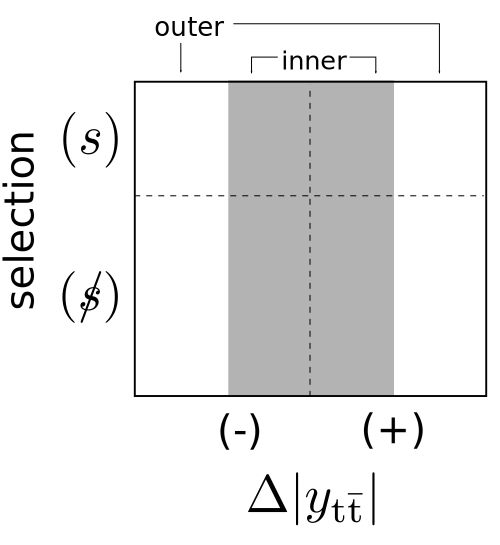
\includegraphics[width=0.4\linewidth]{axes2}
  \caption{\label{axes2} Additional distinction of inner $(\pm)$ bins
    (gray) and outer $(\pm)$ bins (white).}
\end{figure}
We seek to construct a model $M$ possessing the features of model $N$
by specifying differential charge asymmetry and selection efficiency
within the $(\pm)$ bins.  To this end, we specify inner and outer
regions of the $(\pm)$ bins, as shown in Figure \ref{axes2}.  We
choose the number of selected events in the inner and outer bins to be
equal.  The asymmetry in the inner(outer) bins is
$\alpha_{\innr(\outr)}$, independent of selection.  The efficiency in
the inner(outer) bins is $\epsilon_{\innr(\outr)}$, independent of
selection.  After specifying these properties and $\alpha_\selected$,
$\alpha_\tot$, and $N_\selected/(N_\selected+N_\unselected)$, one
degree of freedom remains, which we parameterize with $g$ as
\[\epsilon = \frac{1}{g}\left(\frac{N_\selected}{N_\selected+N_\unselected}\right),\qquad \depsilon=\sqrt{1-g},\qquad\dalpha = \frac{1}{\depsilon}\left(\frac{\alpha_\tot}{\alpha_\selected}-1\right)\]
\[
\begin{array}{r@{\ =\ }l@{,\qquad}r@{\ =\ }l}
  \epsilon_\outr & \epsilon(1 - \depsilon) & \alpha_\outr & \alpha_\selected(1 + \dalpha),\\
  \epsilon_\innr & \epsilon(1+ \depsilon)  & \alpha_\innr & \alpha_\selected(1 - \dalpha).
\end{array}
\]
Figures \ref{diff_eff} and \ref{diff_alp} show
$(\epsilon_\outr,\epsilon_\innr)$ and $(\alpha_\outr,\alpha_\innr)$
parametrizd by $g$ based on POWHEG $\mathrm{t\bar{t}}$. Rebinning
$M(g)$ yields $N=T(1)=U(0)$, so a a two-bin extrapolation of the total
asymmetry from the selection via either unfolding or templates
correctly yields $\alpha_\tot$.  Perturbations of $M(g)$ via scaling
either or both of $\alpha_\innr$ and $\alpha_\outr$ result in a new
total asymmetry $\alpha\ne\alpha_0$.  The two-bin extrapolations are
both (almost, in case of unfolding) linear in $\alpha$ for all three
types of scalings, the slopes of which are shown as a function of
$\epsilon_\innr$ in Figure \ref{diff_slope}.  A slope of 1 indicates
correct extrapolation.  Figure \ref{diff_mistake} shows the
extrapolation mistake relative to $\alpha_\tot$ of flipping the sign
of asymmetry.
\begin{figure}
  \centering
  \subfloat[\label{diff_eff}]{\includegraphics[width=0.5\textwidth,page=1]{plot2}}%
  \subfloat[\label{diff_alp}]{\includegraphics[width=0.5\textwidth,page=2]{plot2}}\\
  \subfloat[\label{diff_slope}]{\includegraphics[width=0.5\textwidth,page=3]{plot2}}%
  \subfloat[\label{diff_mistake}]{\includegraphics[width=0.5\textwidth,page=4]{plot2}}
  \caption{\label{differential} Figures \protect\subref{diff_eff} and
    \protect\subref{diff_alp} show the possible values of inner and
    outer efficiencies and asymmetries in models $M(g)$ for plausible
    $\alpha_\selected$ (0.32\%), $\alpha_\tot$ (0.56\%), and selection
    efficiency (10\%).  Figure \protect\subref{diff_slope} and shows
    the slope of 2-bin extrapolated asymmetry versus 4-bin model
    asymmetry for scaling perturbations of inner, outer, or both inner
    and outer asymmetries.  A slope of 1 implies correct
    extrapolation.  Figure \protect\subref{diff_mistake} shows the
    extrapolation mistake relative to the standard asymmetry of
    flipping the sign of the asymmetry inner/outer/both asymmetry.
    The range between the arrows is more realistic because it does not
    depend sensitively on cancelation of diverging asymmetries from
    inner and outer bins.}
\end{figure}


\section{Reconstruction effects}

Suppose the resolution with which we measure the observable in bins
$(\pm)$ is less than perfect, so that the distribution we record is
$(\pm')$, with a probability $p^{\pm\pm}$ of $(\pm)$ events falling in
$(\pm')$, and $1-p^{\pm\pm}$ of $(\pm)$ events falling in $(\mp')$.
The asymmetry of the observed distribution is
\begin{eqnarray*}
  \alpha'_\selected 
  &=& \frac{N^{+'}_\selected-N^{-'}_\selected}{N_s}\\
  &=& \frac{N^+_\selected p^{++}+N^-_\selected(1-p^{--}) - N^-_\selected p^{--} - N^+_\selected(1-p^{++}) }{N_\selected}\\
  &=& \frac{N^+_\selected(2p^{++}-1) - N^-_\selected (2 p^{--} - 1) }{N_\selected}.
\end{eqnarray*}
Only if there is no asymmetry introduced in reconstructing the
observable, so that $p^{++}=p^{--}=p$, is $\alpha'_\selected$
proportional to $\alpha_\selected$,
\[\alpha'_\selected = \alpha_\selected(2p-1),\]
so that scaling of $\alpha_\selected$ propogates exactly to
$\alpha'_\selected$.  In general, the antisymmetric component of a
smeared distribution will scale by the factor applied to the
antisymmetric component of the unsmeared distribution, as long as the
smearing itself is symmetric.


\end{document}
